
\chapter{Introductions and Basics}
\label{chpt:intro2Classs}

\section{Partial Differential Equations Overview}

There are three classic partial differential equations (PDEs):

\vspace{0.5em}

\hspace{2em} \textbf{I.}  Wave equation: \hspace{5.5em} $\nabla^2 \phi = \dfrac{1}{c^2} \dfrac{\partial^2 \phi}{\partial t^2} $  \hspace{2.2em} \emph{(hyperbolic)}

\vspace{0.8em}

\hspace{2em}  \textbf{II.}  Heat/diffusion equation: \hspace{1em} $\nabla^2 \phi = \dfrac{1}{k} \dfrac{\partial \phi}{\partial t}$  \hspace{3em} \emph{(parabolic)}

\vspace{0.8em}

\hspace{2em}  \textbf{III.}  Laplace's equation: \hspace{3.2em} $\nabla^2 \phi = 0$  \hspace{4.8em} \emph{(elliptic)}


\noindent Here $\phi$ denotes some property (i.e., velocity, pressure), $t$ time, and $c,k \in \mathbb{R}$ are constants. $\nabla$ is the nabla operator and its definition depends on the context. Generally, $\nabla$  is an $n$-dimensional vector operator whose components contain a partial derivative operation with respect to the dimension of their index. For example,
\begin{align*}
\text{n = 1}: \hspace{1em} \nabla &= \left[ 
\frac{\partial }{\partial x} \right]\\
\text{n = 2}: \hspace{1em} \nabla &= \left[ 
\frac{\partial }{\partial x} \ ,  \ \frac{\partial }{\partial y} \right] \\
\text{n = 3}: \hspace{1em}  \nabla &= \left[ 
\frac{\partial }{\partial x} \ , \ \frac{\partial }{\partial y}, \ \frac{\partial }{\partial z} \right]
\end{align*}

\noindent Let's consider a two-dimensional ($n = 2$) domain $\Omega$ and the property velocity $\mathbf{u} = \left[u(x,y), v(x,y) \right]$, where $(x,y) \in \Omega$. Then,
$$
\nabla \cdot \mathbf{u}= \left[ 
\frac{\partial }{\partial x} \ , \ \frac{\partial }{\partial y} \right] \cdot  \left[  u(x,y), v(x,y) \right]= 
\frac{\partial u(x,y) }{\partial x} + \frac{\partial v(x,y)}{\partial y}.
$$
This is simply the divergence of $\Omega$. The $\nabla$ operator also appears for calculations of gradients ($\nabla \mathbf{u}$) and curl ($\nabla \times \mathbf{u}$).

Each of the three classic PDEs have their own set of applications. The wave equation $\mathbf{I}$ can help model the motion of specific waves, such as sound and electromagnetic, and how they interact with solids. Heat transfer and basic diffusion of chemicals, such as air pollutants, can be modeled with the diffusion equation $\mathbf{II}$. Laplace's equation $\mathbf{III}$ can be applied to gravitational attraction and electrostatics. All of these equations have many more applications than those listed here, but these give applications provide intuition on how they can be used to better understand dynamical systems.

Note that all three of these equations are linear, second-order, homogeneous PDEs. Recall that a PDE is linear if no unknowns are multiplied together, second-order because the highest derivative of $\mathbf{u}$ is two, and homogeneous because it is only an equation of unknowns. In all three, $\mathbf{u} = \mathbf{0}$ is always a solution and the principle of superposition can be applied. These properties allow us to construct many solutions of the PDE by separation of variables. All three equations also contain $\nabla^2$, which follows from physical assumptions. Many modeled phenomena are independent of coordinate system, meaning that the choice or origin and orientation of axes does not change the outcome.  $\nabla^2$ is also independent of the coordinate system, making it a standard choice when modeling these phenomena.

Inhomogeneous versions of classic PDEs are of interest as they allow us to understand how a system behaves when forced. One notable example is Poisson's equation
$$
\nabla^2 \phi = \mathbf{f},
$$
where $f$ is a given function and $\phi$ is unknown. Often we cannot solve these by hand, leading to the development of numerical methods. Numerical methods fall into two main categories: colocation and Galerkin. Colocation methods solve for $\phi$ at discrete points across the domain. Galerkin methods rely on known basis functions and solve for $\phi$ in terms of these bases. In this class, we will consider

{
\centering
\begin{enumerate}
\item Finite difference methods (Colocation)
\item Finite element methods (Galerkin)
\item pseudo-spectral methods (either)
\item boundary integral methods (either)

\end{enumerate}
}

\section{How to Visually Communicate}
\label{chpt:visComm}


 Pictures, figures, images, plots, etc. are all forms of visual communication. Any visual communication should be made in the most \textit{effective} and \textit{accessible} way possible. This chapter will discuss what it means to visually communicate effectively and ensure accessibility when creating line and field plots from data. General implementation of these practices in python and MATLAB is provided in Section~\ref{chpt:figCode}. 

\index{plotting}
\index{figure making}

\subsection{Effective and Accessible Communication}
\label{chpt:effectiveFigs}
Visual communication is effective when the reader immediately understands what is being presented. Labels, such as those in legends and on axes, informs the reader without the need for questions, assumptions or guessing. Units for the axes set the scale of the problem, which allows the reader to understand physical or numerical implications without explanation. Captions describe the visualization in words and include what the reader needs to understand the plot's labels, such as variable definitions. Note that conclusions or analysis \textit{should not} be discussed in captions. Plots can imply if the data are discrete or continuous through style; data are generally discrete and should be plotted using symbols, while theory/fits should be plotted as continuous curves. All of these choices discussed make visual communication more effective.

For visual communication to be completely accessible, no reader should be at a disadvantage due to physical abilities or technological access. Colorblindness can make data difficult to discern if the colors do not contrast, especially when considering those who are completely colorblind or when work is printed in black and white. Efforts to use more than color, such as markers, and to select contrasting colors ensure general readability no matter the case. Assistive technology is capable of converting visual communication to non-visual communication by reading alternative text of images. Although out of the scope of this class, it is important to include and use descriptive alternative text so that any visual communication can be understood without seeing the image or figure. 

The next two subsections will discuss class standards on visual communication for line and field plots. Code used to produce Figures~\ref{fig:lineExample} and \ref{fig:exampleFields} is provided in Section~\ref{chpt:figCode}.

\newpage
\subsubsection{Line Plots}
Consider the presentation of data in Figure~\ref{fig:lineExample}. The figure is arranged in two columns: column (1), on the left, shows a poorly made plot, while column (2), on the right, shows a well-constructed plot. The three rows \emph{(a)}, \emph{(b)}, and \emph{(c)} correspond to three different color spectrums: full RGB, that related to protanopia (red-green colorblind), and grayscale. Table~\ref{tab:lineComparison} compares each flaw of plot (1) with its correction in column (2), with a description of how the correction increases effectiveness in column (3).
\begin{table}[h!]
    \centering
    \begin{tabular}{|>{\raggedright\arraybackslash}p{3cm}|>{\raggedright\arraybackslash}p{4cm}||>{\raggedright\arraybackslash}p{6cm}|}
        \hline
        \textit{Bad plot traits (seen in 1)} & \textit{Good plot traits \ \ \ \ \ \ \ \  (seen in 2)} & \textit{Impact to reader} \\
        \hline
        No data symbols & Large, differentiable data symbols & Shows where the data actually is. \textbf{Symbols represent data; curves represent theory/fits.} {\small Symbols also keep data distinguishable in the legend and plot when color fails (e.g., poor projector or paper printout).} \\
        Small tick labels (numbers on axes) & Large labels everywhere & \textbf{Make everything larger than you think!} Easier for the viewer to read and interpret the data. \\
        No labels for data, plot, or axes & Fully labeled plot \textbf{with units} & Tells the reader what is being presented and the scale of the problem. \\
        Similar colors for different data & Unique, contrasting colors for each dataset & Keeps data distinguishable for colorblind readers and in grayscale, shown in plots (b) and (c). Similar RGB colors can become identical in both cases. \\
        Linearly scaled axes & Logarithmically scaled axes & Reveals power-law behavior. \\
        No reference lines & Reference lines for $n$-order convergence & Confirms to the reader that the claimed order of convergence is actually achieved. \\
        Programs default font (mismatched with document) & Font matching the document body (e.g., Latin Modern) & Makes plot text consistent with the surrounding \LaTeX{} type, so figures don't look pasted in. \textbf{Computer/Latin Modern or Helvetica/Free Sans are strongly recommended.} \\
        \hline
    \end{tabular}
    \caption{Description of differences in plots shown in Figure~\ref{fig:lineExample} and their impact on readability.}
    \label{tab:lineComparison}
\end{table}

\clearpage
\newpage


\begin{figure}[!ht]
\begin{framed}
  % ---- Row 1 ----
  \emph{1}(\emph{a})
  \hspace*{7cm}
  \emph{2}(\emph{a})\\
  \hspace*{5mm}
  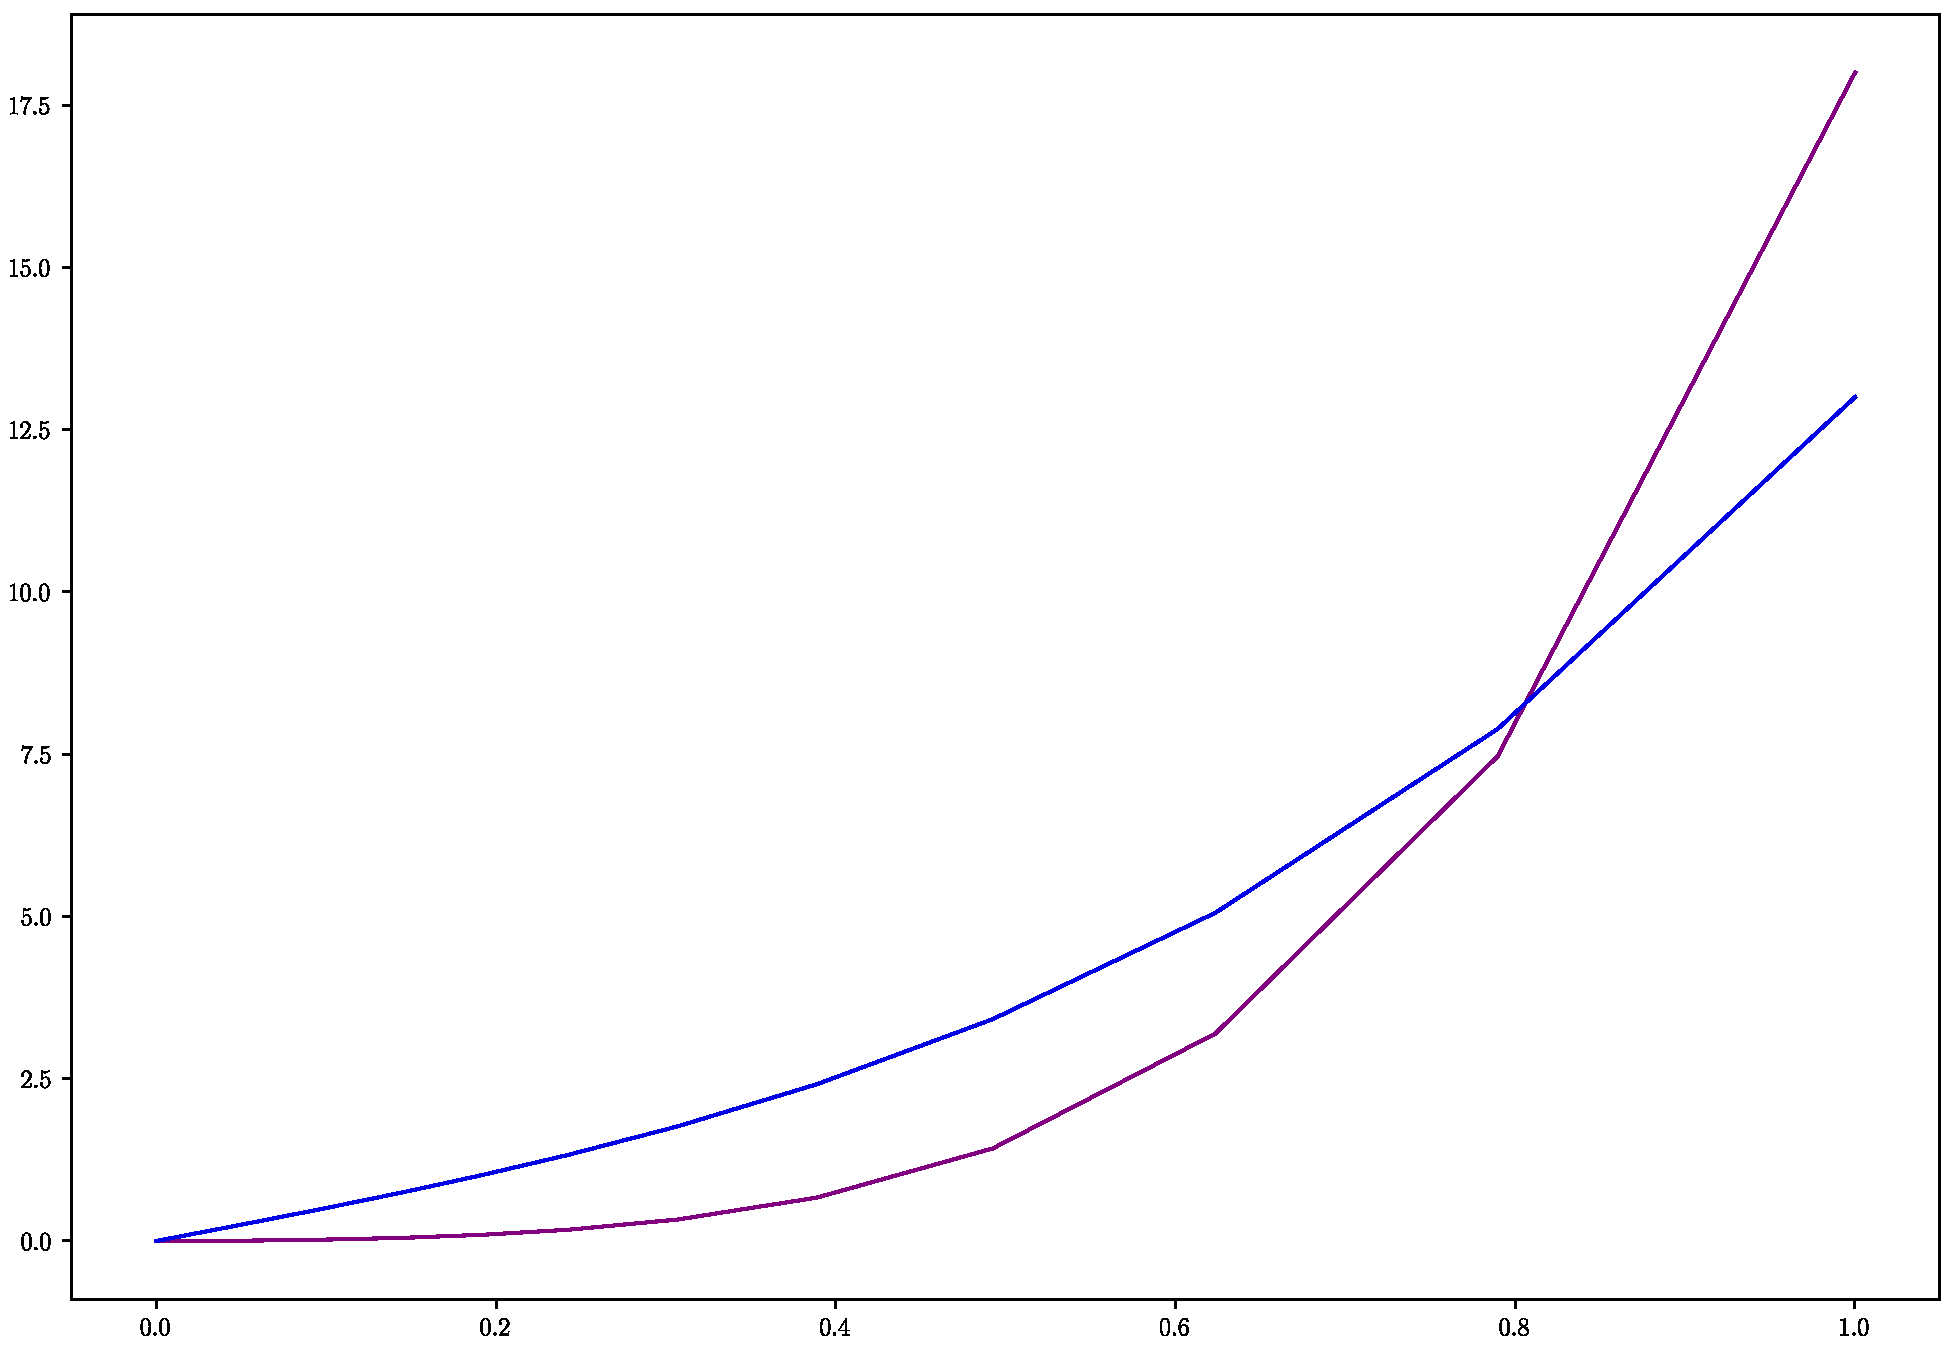
\includegraphics[trim = 0mm 0mm 0mm 0mm,clip,
  width=7.0cm, page=1]{Plots/images/linesv5.pdf}
  \includegraphics[trim = 0mm 0mm 0mm 0mm,clip,
  width=7.0cm, page=4]{Plots/images/linesv5.pdf}\\[2mm]
  % ---- Row 2 ----
  \emph{1}(\emph{b})
  \hspace*{7cm}
  \emph{2}(\emph{b})\\
  \hspace*{5mm}
  \includegraphics[trim = 0mm 0mm 0mm 0mm,clip,
  width=7.0cm, page=2]{Plots/images/linesv5.pdf}
  \includegraphics[trim = 0mm 0mm 0mm 0mm,clip,
  width=7.0cm, page=5]{Plots/images/linesv5.pdf}\\[2mm]
  % ---- Row 3 ----
  \emph{1}(\emph{c})
  \hspace*{7cm}
  \emph{2}(\emph{c})\\
  \hspace*{5mm}
  \includegraphics[trim = 0mm 0mm 0mm 0mm,clip,
  width=7.0cm, page=3]{Plots/images/linesv5.pdf}
  \includegraphics[trim = 0mm 0mm 0mm 0mm,clip,
  width=7.0cm, page=6]{Plots/images/linesv5.pdf}\\[2mm]
  \caption{Column 1 and Column 2 represent line plots of the same dataset with different plotting styles. The three rows \emph{(a)}, \emph{(b)}, and \emph{(c)} correspond to full RGB color, color as experienced with protanopia (red–green colorblindness), and grayscale, respectively.}
  \vspace*{2mm}
    \label{fig:lineExample}
\end{framed}

\end{figure}


\clearpage 
\newpage
\subsubsection{Field Plots}


Plotting fields is an effective way to understand what a system is doing at an instance of time.  Efforts to make fields more effective and accessible are focused on ensuring the labels are clear and a good colormap is selected. 

\begin{figure}[!ht]
    \centering
    
\includegraphics[width=0.75\linewidth]{Plots/images/blues.jpg}\\ [4mm]
    % \hspace{6cm}
    % \vspace{1cm}
    
\includegraphics[width=0.75\linewidth]{Plots/images/curl.jpg}
    \caption{A sequential colormap (\textit{blues}) on top and a diverging colormap (\textit{curl}) on bottom. Images from \textcite{cmapRepo}.}
    \label{fig:exampleCMs}
\end{figure}

A colormap is a gradient of color, as seen in Figure~\ref{fig:exampleCMs}. Colormaps map numerical values of a field to colors along a gradient, which allows for spatial visualization of variations of the field. Different styles of colormap suit different applications; here we consider \textit{sequential} and \textit{divergent} maps.


Sequential colormaps change monotonically from one end to the other, like the \textit{blues} map at the top of Figure~\ref{fig:exampleCMs}, which runs from dark blue to bright white. Sequential maps are effective for fields where growth or subtle changes in magnitude across the field are important to discern.

Divergent colormaps change monotonically from each end toward the middle, where two dark colors meet at a bright center, as in the \textit{curl} \parencite{cmoceanRep} map shown at the bottom of Figure~\ref{fig:exampleCMs}. Divergent maps are effective for highlighting variation from means in fields that diverge or cycle around a value (i.e., sinusoidal).


Consider the two-dimensional fields shown in Figure~\ref{fig:exampleFields}. The field in column 1 is considered sequential, as the data grows monotonically to peaks at different points in the field. The field is column two contains discontinuous oscillations about $f(x,y) = 0$. A divergent color map clearly shows where these oscillations are and the general pattern they have across the field, while highlighting the mean. This pattern is much more apparent in the two-dimensional (2D) plot (2b), whereas the three-dimensional (3D) plot (2b) does not accurately reflect the field. In this case, the field at the center is hidden by the large magnitude oscillations along the $x$ axis. In 1(b), it is not clear what is happening behind the peaks of the field. These examples highlight the importance of angle at which the data is plot, as the surface can hid information when certain angles are chosen. Generally, it is best to plot in 2D to ensure a full view of the data field, as seen in the (a) row of Figure~\ref{fig:exampleFields}.

 \begin{figure}[htbp]
\begin{framed}
  % ---- Row 1 ----
  \emph{1}(\emph{a})
  \hspace*{7cm}
  \emph{2}(\emph{a})\\
  \hspace*{5mm}
  \includegraphics[trim = 0mm 0mm 0mm 0mm,clip,
  width=7.0cm]{Plots/images/compCMAPSeqFlat.pdf}
  \includegraphics[trim = 0mm 0mm 0mm 0mm,clip,
  width=7.0cm]{Plots/images/compCMAPDivFlat.pdf}\\[2mm]
  % ---- Row 2 ----
  \emph{1}(\emph{b})
  \hspace*{7cm}
  \emph{2}(\emph{b})\\
  \hspace*{5mm}
  \includegraphics[trim = 0mm 0mm 0mm 0mm,clip,
  width=7.0cm, page=2]{Plots/images/compCMAP3D.pdf}
  \includegraphics[trim = 0mm 0mm 0mm 0mm,clip,
  width=7.0cm, page=1]{Plots/images/compCMAP3D.pdf}\\[2mm]
  \caption{Column 1 and Column 2 represent field plots of the same dataset with different plotting styles. The two rows \emph{(a)} and \emph{(b)} correspond to flat pseudocolor plots and 3D plots, respectively.}
  \label{fig:exampleFields}
  \vspace*{2mm}
\end{framed}
\end{figure}


\clearpage

\newpage

What makes a colormap good? Color can mean more than just showcasing subtle changes or disparities around a mean. It can help showcase landscapes, simulations of ocean surfaces, statistical disparities, and much more. Many colormaps are born from a need to have both effective and accessible visual communication in situations that call for certain color schemes or styles. Open-source colormap repositories include:

\begin{itemize}
\item  cmocean \parencite{cmoceanRep, cmoceanarticle}: for presenting oceanography data, \\
\item \textit{CMasher} \parencite{cmasher}: aimed for making accessible, informative, and \textit{cmashing} plots \\
\item  seaborn \parencite{seaborn}: for statistical data visualization \\
\item cmap \parencite{cmapRepo}: perceptually uniform colormaps for MATLAB, compiled from multiple sources. \\
\item scientific \parencite{scientific}: accurate data visualization needs and accurate scales readable by everyone. 
\end{itemize}

Some colormaps can fall into more than one category as well, making them effective tools in general cases. \textit{turbo}\parencite{turboCM} is one of the most popular colormaps because it can be applied to many different styles of data effectively and was designed with accessibility in mind. 

\begin{figure}[!ht]
\centering
    
\includegraphics[width=0.75\linewidth]{Plots/images/jet.jpg}\\ [2mm]
    
\includegraphics[width=0.75\linewidth]{Plots/images/turbo.jpg}\\ 
    \caption{jet (top) and turbo (bottom), both sequential and diverging colormaps. turbo image from \textcite{cmapRepo}.}
    \label{fig:turboCM}
 \end{figure}
 
\textit{turbo}, shown at the bottom of Figure~\ref{fig:turboCM}, is a form of rainbow colormap. \textit{tubo} was created to address major faults in \textit{jet}, the top color map of Figure~\ref{fig:turboCM}. \textit{jet} is high in contrast and has distinct color bands which manifest on data, making certain areas seem less smooth than they are. This phenomena is known as "false detail" and should be considered when picking a colormap. The left tail on \textit{jet} is a broad, almost-uniform blue gradient that manifests as one color in grayscale and for the colorblind, making it inaccessible. \textit{turbo} addresses these problems with a perceptually uniform rainbow with well-defined tails, effectively removing the false detail, color bands, and inaccessibility concerns of \textit{jet}. 

These rainbow maps are unique as they serve as both sequential and divergent colormaps. They are particularly popular showing details across a range of magnitudes, as the combination of style highlights extremes at both end points and in the middle. Application of rainbow plots to study depth in images allows information at the far-field and near-field to be highlighted without overlooking what lies between. 

We analyze \textit{jet} and \textit{turbo} in Figure~\ref{fig:dispair}, which showcases an image of a road in three sets of three. In each set, three colormaps are applied to the image: \textit{cool}, \textit{jet}, and \textit{turbo}. Each set is then displayed in three different color spectrums: full RGB, that related to protanopia (red-green colorblind), and grayscale. Consider a case where it is important to have information up-close and far away, but also to clearly see when something stands out. One example might be a self-driving car analyzing its path ahead, where it needs to know where it is, whats coming ahead, and if there is something along the path, like a person crossing the road or another car.

Looking at the full RGB set (set 1), it is clear that \textit{cool} (top image) captures only the closest cars, with everything at a distance either vague or washed out. The ability of \textit{jet} (middle) to capture detail is clear, with street posts and cars even at long-distance standing out. However strong color bands are seen on the closer cars and everything at a certain distance has similar colors of blue.  In comparison, \textit{turbo} (bottom) has smooth gradients on the closest cars, the further perceived depth, and builds on the sharp detail of \textit{jet} for all distances.

Sets 2 and 3 showcase the same images as set 1 but for the color scale of protanopia (red-green colorblindness) and a grayscale, respectively. In set 2, \textit{cool} does not change much, which follows as there is minimal red and green, but shows its flaws in the grayscale of set 3 where the image is completely gray with no detail.  \textit{jet} has more detail stand out at a distance for set 2, with the blues becoming more defined than in RBG, but the color bars on the closet cars expand. At grayscale, \textit{jet} is able to maintain a lot of detail but fails to maintain a uniform gradient, making it hard to tell depth without perspective of the objects on the street. \textit{turbo} is able to maintain detail at a distance in both set 2 and 3, but loses some of its uniform gradient at grayscale with closer details blending together. 

This discussion of colormaps highlights that certain colormaps are effective for specific data analysis and considerations for unconventional RBG scales makes visual communication of that data more accessible to all. In this class, data will generally be either sequential or divergent. Choosing colors that relate to the problem (i.e., \textit{Blues} for water) should be considered, while keeping in mind that not all colors are accessible. 


 


\begin{figure}[!ht]
\begin{framed}
\centering
\setlength{\tabcolsep}{2pt}
\begin{tabular}{c c}
  % ---- Row 1 ----
  \rotatebox{90}{\makebox[6cm][c]{\emph{Set 1: full RGB}}}
  & 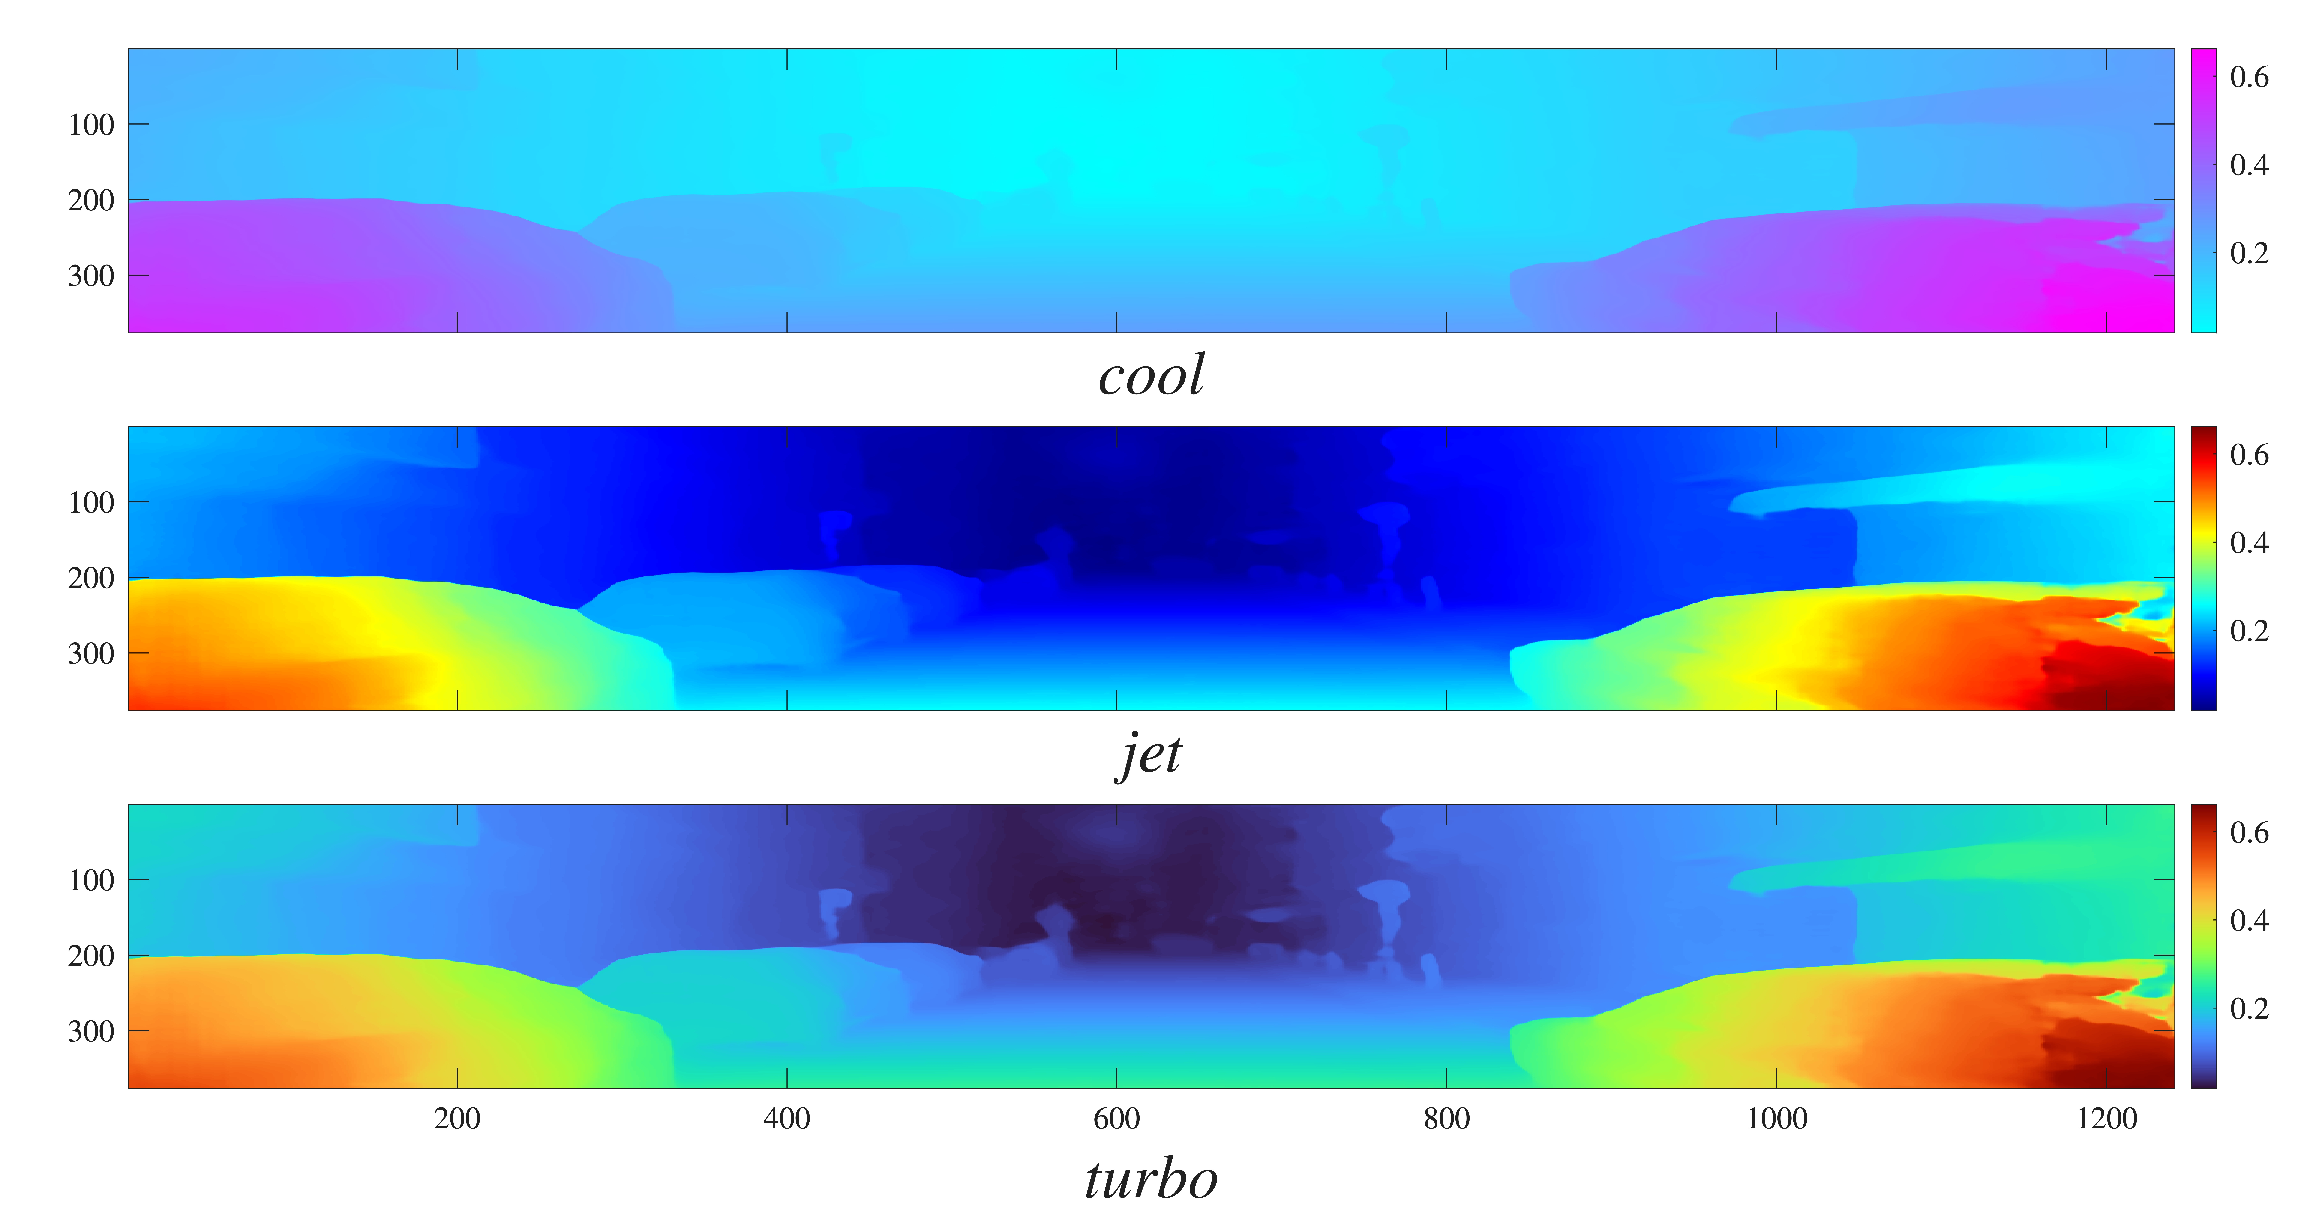
\includegraphics[width=0.80\linewidth]{Plots/images/dispRBG.pdf} \\
  % ---- Row 2 ----
  \rotatebox{90}{\makebox[6cm][c]{\emph{Set 2: protanopia}}}
  & 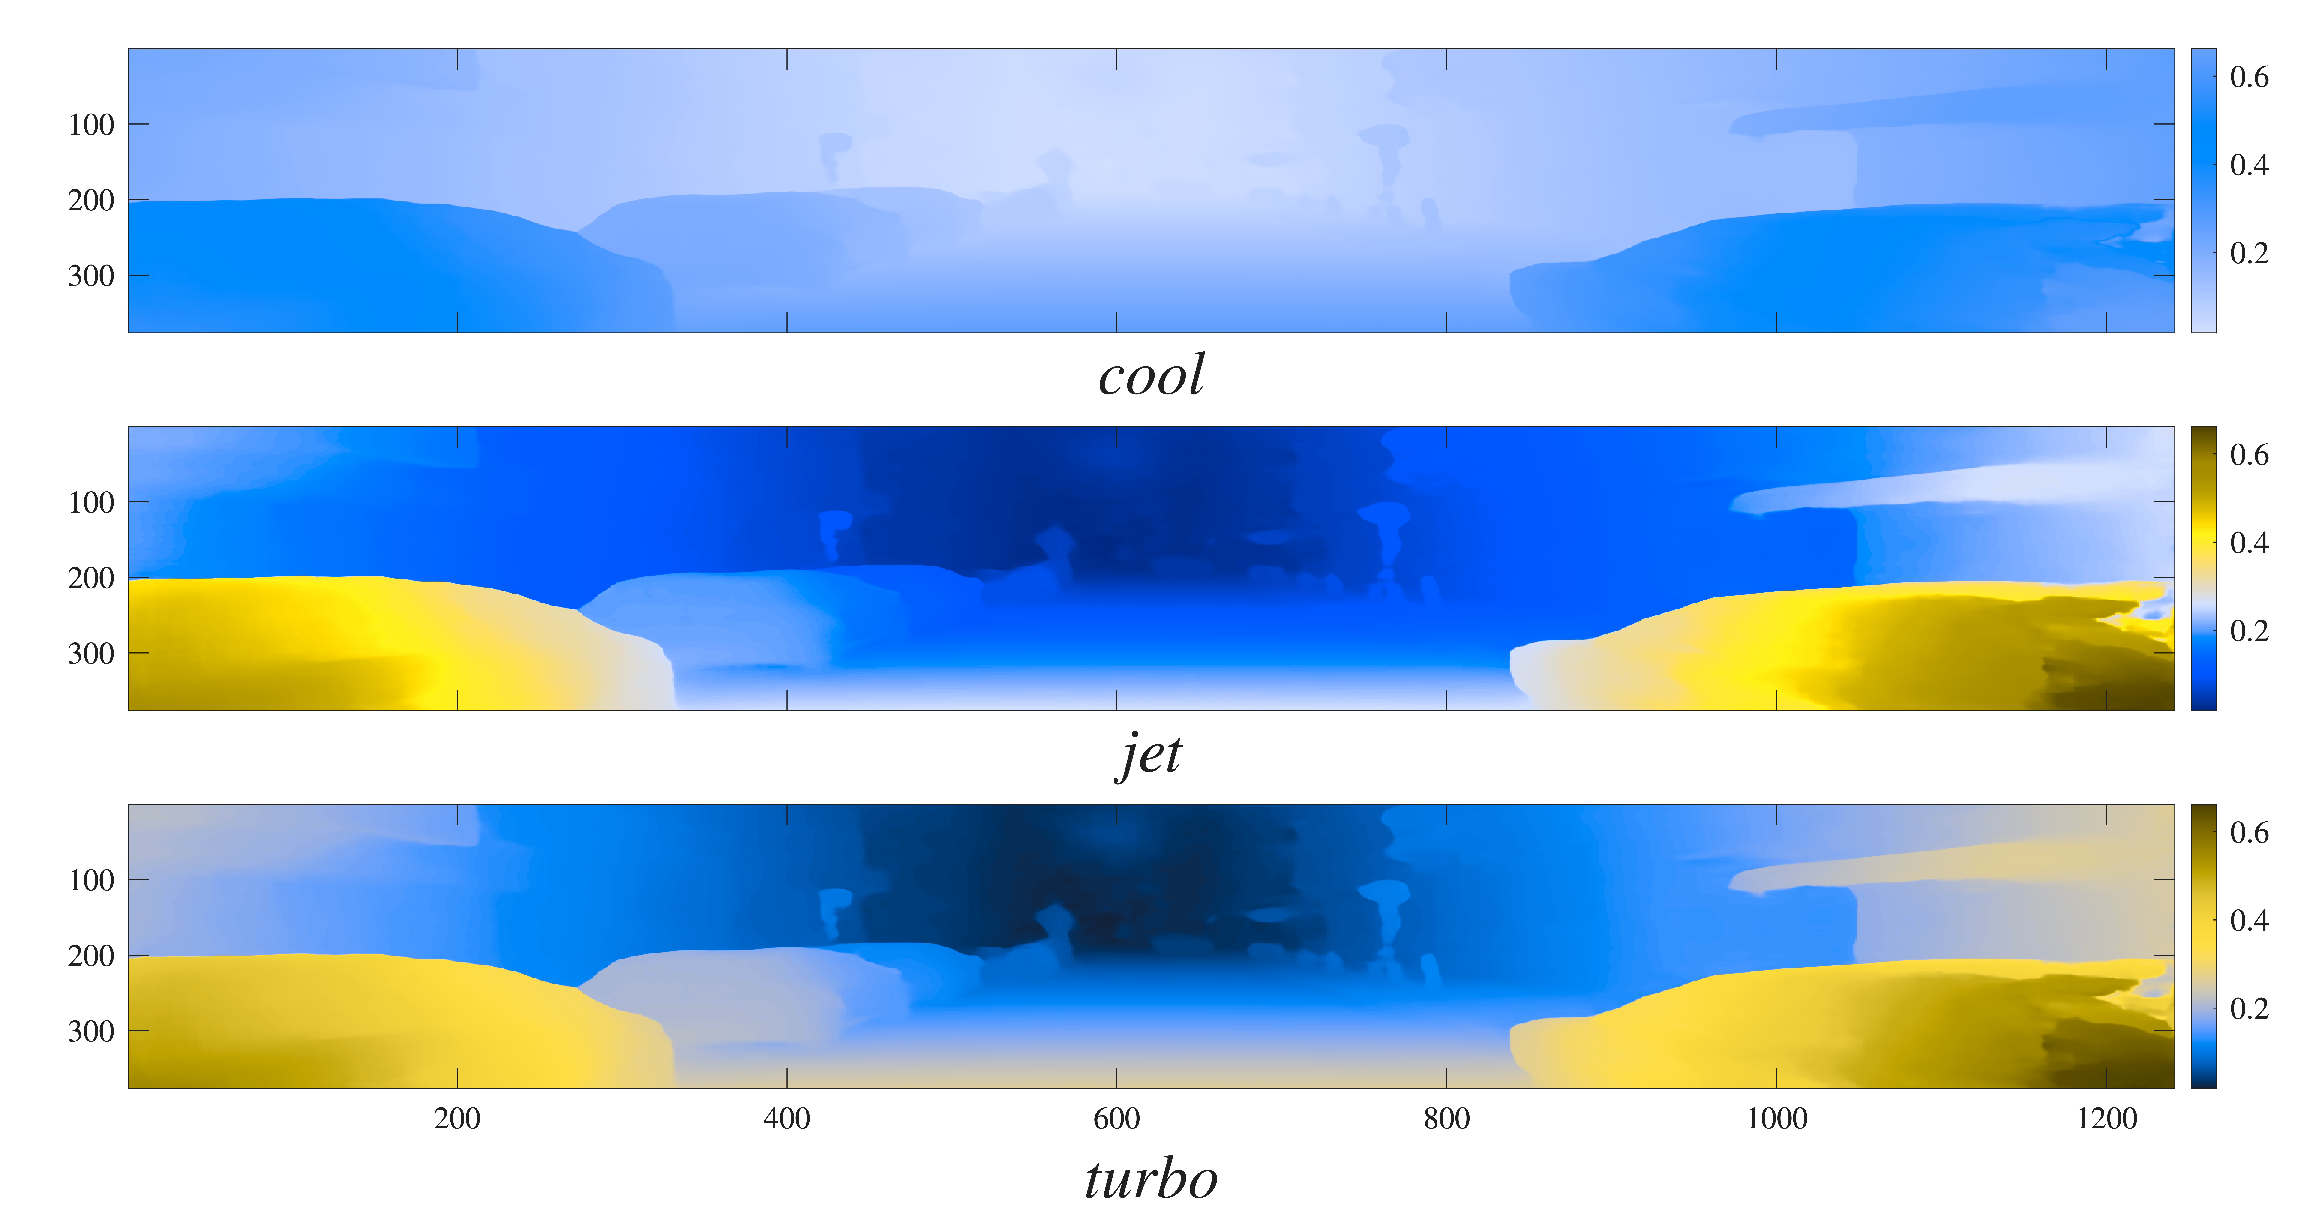
\includegraphics[width=0.80\linewidth]{Plots/images/dispProton.pdf} \\
  % ---- Row 3 ----
  \rotatebox{90}{\makebox[6cm][c]{\emph{Set 3: grayscale}}}
  & 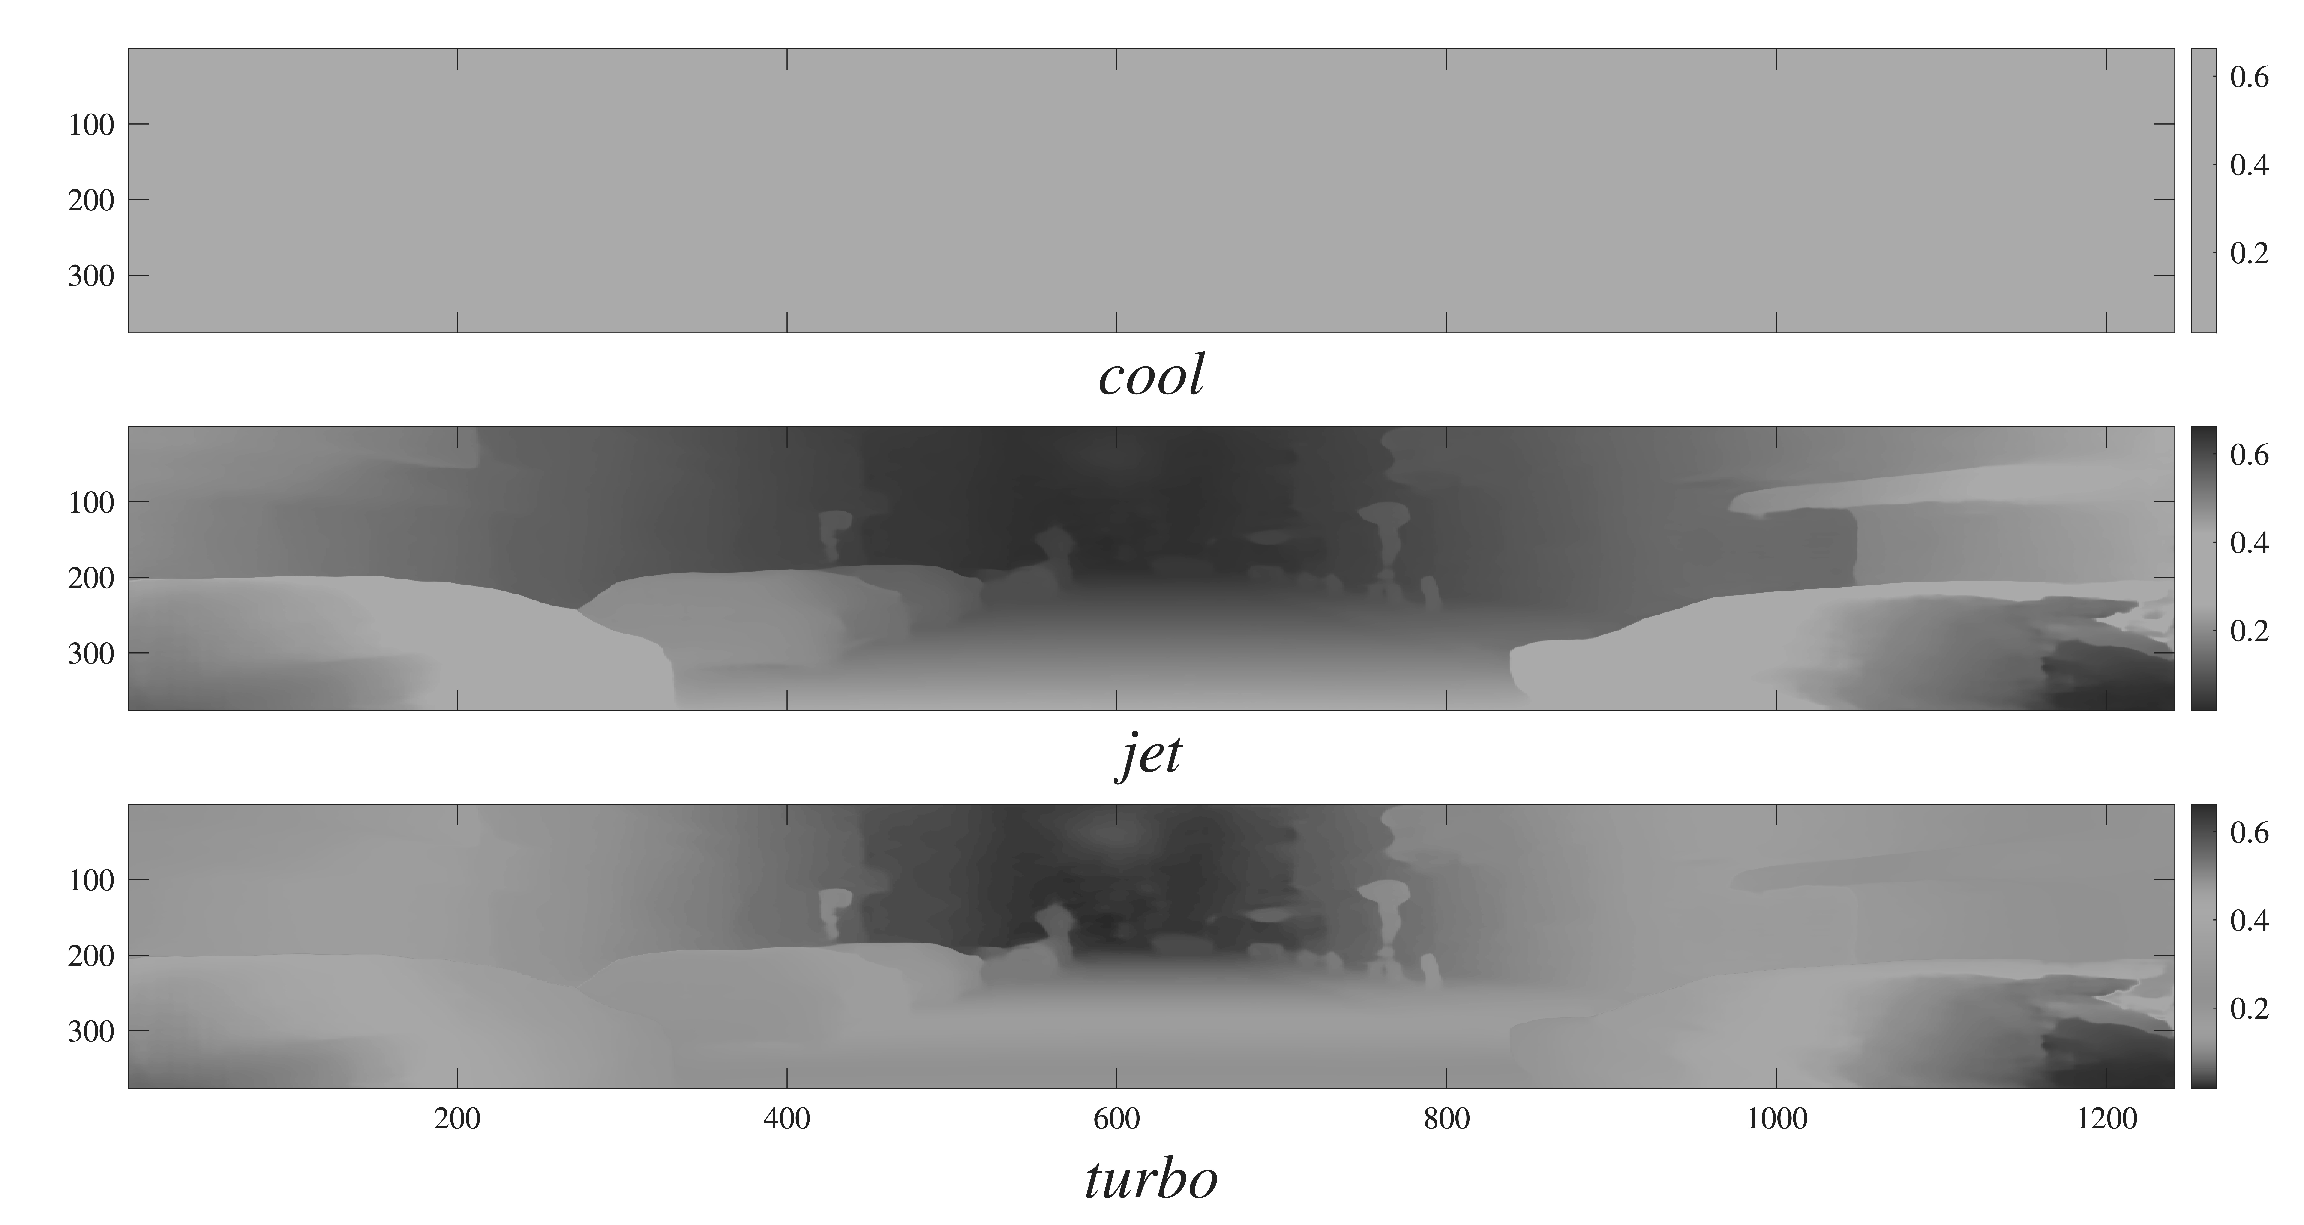
\includegraphics[width=0.80\linewidth]{Plots/images/dispMono.pdf} \\
\end{tabular}
\caption{An image of a road in three sets of three. The main set is three colormaps applied to the image: \textit{cool}, \textit{jet}, and \textit{turbo}. This set is then showcased for three different color spectrums: full RGB (Set 1), that related to protanopia/red-green colorblind (Set 2), and grayscale (Set 3).}
\label{fig:dispair}
\end{framed}
\end{figure}
 
 

% { \Large \textcolor{magenta}{fix caption and once thats decided make as big as possible ALSO READ THRU CODE TO QC} }

\clearpage

% Now, let's consider . Each row of showcases the same data as that in  Figure~\ref{fig:exampField}, but with different colormaps. When choosing colormaps, it is important to consider both what is being presented and if the map is accessible. You may be drawn to the \textit{ice} colormap shown in row 1, as blue is a natural color choice for fluid or you enjoy it. However, \textit{ice} in grayscale washes out the gradient between the rings of "waves", making the field look more binary than connected. Row 2 shows \textit{jet}, once a quite popular colormap. You'll   

\subsection{Implementations}
\label{chpt:figCode}

{
\centering
\subsubsection{Lines in python}
\hrule{}
}

\begin{lstlisting}[language=python]
# plotting package import
import matplotlib.pyplot as plt
# numerics package import
import numpy as np

# LaTeX rendering in Latin Modern
plt.rcParams['text.usetex'] = True
plt.rcParams['text.latex.preamble'] = r'\usepackage{lmodern}'
plt.rcParams['font.family'] = 'serif'

# generate data
dxs = np.logspace(-4, 0, 40)  # grid spacings, 10^-4 to 10^0
y1 = 5.0*(dxs) + 8.0*(dxs**3)     # first order error curve
y2 = 2.0*(dxs**2) + 16.0*(dxs**4) # second order error curve

# reference lines (order one ref. is just dxs itself)
ref2 = dxs**2  # order two reference line

fs = 50  # set font size variable

# this is how you define non-standard colors! 
# all these values are the RBG #/255. this accepts both the 
# calculation (67/255) and the fraction (0.2627) for RBG triplets (see below)
badCols = np.array([
    [0.5, 0.000, 0.5],  # purple
    [0, 0, 0.9],        # blue
])

cols = np.array([
    [67/255, 179/255, 174/255],   # teal (marker edge/line 1)
    [136/255, 216/255, 192/255],  # light green (marker face 1)
    [198/255, 97/255, 166/255],   # light magenta (marker face 2)
    [202/255, 44/255, 146/255],   # magenta (marker edge/line 2)
])

# define figure, axes, and size
fig, ax = plt.subplots(figsize=(13, 9))

# bad color choice example (uses badCols)
# ax.plot(dxs, y1, '-', color=badCols[0, :])
# ax.plot(dxs, y2, '-', color=badCols[1, :])

# reference lines (excluded from legend)
ax.plot(dxs[:20], dxs[:20], '-.', color='black',
        linewidth=5, 
        label='_nolegend_') # this excludes this line from the legend
ax.plot(dxs[:20], 0.3*ref2[:20], '--', color='black',
        linewidth=5, label='_nolegend_')

# plots y1 vs dxs every third point as solid line with markers
ax.plot(dxs[::3], y1[::3], '-o',
        color=cols[0, :],            # set line color
        linewidth=2,                 # set line width
        markersize=24,               # set marker size
        markeredgewidth=3,           # set marker outline width
        markeredgecolor=cols[0, :],  # set marker outline color
        markerfacecolor=cols[1, :],  # set marker fill color
        label='first order')         # set legend entry

ax.plot(dxs[::3], y2[::3], '-*', color=cols[3, :], linewidth=2,
        markersize=40, markeredgewidth=3, markeredgecolor=cols[3, :],
        markerfacecolor=cols[2, :], label='second order')

# label reference slopes directly on the plot
ax.annotate(r'$\mathcal{O}(\Delta x)$',
            (1.3*dxs[5], 0.3*dxs[5]), fontsize=0.75*fs)
ax.annotate(r'$\mathcal{O}(\Delta x^2)$',
            (2.3*dxs[5], 0.4*(dxs[5]**2)), fontsize=0.75*fs)

# the multiplications you see above are simply translating the position to get 
# the labels off the line but close to it!

for spine in ax.spines.values():  # set axes line width
    spine.set_linewidth(3)
ax.tick_params(width=3, labelsize=fs)  # set tick width and font size
ax.tick_params(axis='x', pad=10)       # pad ticks away from axis (preventing overlap)

ax.set_xlabel(r'$\Delta x$  (mm)', fontsize=fs, labelpad=2)
ax.set_ylabel(r'Error', fontsize=fs)

ax.legend(fontsize=0.75*fs, loc='lower right')
ax.set_title('Convergence Plot', fontsize=fs)

# set the axis scale to log log
ax.set_xscale('log')
ax.set_yscale('log')
ax.grid() # sets major grid lines - can have settings here

plt.show()  

## note: fig will not save if plt.show() is before plt.savefig(...)!!!!
# plt.savefig("linePlotExample.pdf", dpi=800)  # uncomment to export figure (dpi sets raster resolution)
\end{lstlisting}

{
\centering
\subsubsection{Fields in python}
\hrule
}

 \begin{lstlisting}[language=python]
# plotting package import
import matplotlib.pyplot as plt
# numerics package import
import numpy as np
# import nicer colormaps
import cmocean

# LaTeX rendering in Latin Modern
plt.rcParams['text.usetex'] = True
plt.rcParams['text.latex.preamble'] = r'\usepackage{lmodern}'
plt.rcParams['font.family'] = 'serif'

# generate data
dx = 0.01
x = np.arange(-np.pi, np.pi + dx, dx)  # + dx includes endpoint
y = x
X, Y = np.meshgrid(x, y) # creates mesh of x and y (2D fields)

# diverging colormap example (use cmap='cmo.curl' in pcolormesh)
###########################################################
R = np.sqrt(X**2 + Y**2)
f = Y * np.sin(2.0 * R**2)
###########################################################

# sequential colormap example (use cmap='Blues' in pcolormesh)
###########################################################
# f = R * 1.3**(1.01*(abs(abs(X)*abs(Y) - 2*np.pi)) + np.pi/2)
###########################################################

fs = 35  # set font size variable
cm = 'cmo.curl' # 'Blues'

fig, ax = plt.subplots(figsize=(12, 9))  # set figure size

ax.set_aspect('equal')  # force square aspect ratio

# pseudocolor plot of f across X and Y
# gouraud shading interpolates between cells (no mesh lines)
pc = ax.pcolormesh(X, Y, f, cmap=cm, shading='gouraud')

ax.set_xlabel('$x$', fontsize=fs)  # label x-axis in latex
ax.set_ylabel('$y$', fontsize=fs)  # label y-axis in latex

for spine in ax.spines.values():  # set axes line width
    spine.set_linewidth(3)
ax.tick_params(width=3, labelsize=fs)  # set tick width and font size

axesLims = [-np.pi, np.pi]  # define axes limits
ax.set_xlim(axesLims)       # set x axis limits
ax.set_ylim(axesLims)       # set y axis limits

cb = fig.colorbar(pc, ax=ax)                  # add colorbar
cb.ax.tick_params(labelsize=fs)               # set colorbar tick size
cb.set_label('Field Magnitude', fontsize=fs)  # label colorbar

# tick locations and latex labels
ticks = [-np.pi, -np.pi/2, 0, np.pi/2, np.pi]
tickLabel = ['$-\\pi$', '$-\\pi/2$', '$0$', '$\\pi/2$', '$\\pi$']
ax.set_xticks(ticks)           # set x tick locations
ax.set_yticks(ticks)           # set y tick locations
ax.set_xticklabels(tickLabel)  # set x tick labels to tex strings
ax.set_yticklabels(tickLabel)  # set y tick labels to tex strings

# plt.show()  # uncomment to view interactively

## note: fig will not save if plt.show() is before plt.savefig(...)!!!!
# plt.savefig("divergencePlotExample.pdf", dpi=800)  # uncomment to export figure 
# (dpi sets raster resolution)

#### 3D Plot

fig, ax = plt.subplots(subplot_kw={"projection": "3d"}, figsize=(12,9))

ax.plot_surface(X, Y, f, cmap=cm)

fs = 0.8*fs

ticks = [-np.pi, -np.pi/2, 0, np.pi/2, np.pi]  # defining location of ticks
tickLabel = ['$-\\pi$', '$-\\pi/2$', '$0$', '$\\pi/2$', '$\\pi$']  # defining labels for ticks

ax.set_xticks(ticks)            # set x ticks to ticks array
ax.set_yticks(ticks)            # set y ticks to ticks array
ax.set_xticklabels(tickLabel)   # set labels to tex strings in tickLabel
ax.set_yticklabels(tickLabel)   # set labels to tex strings in tickLabel

ax.set_xlabel('$x$', fontsize=fs, labelpad=20)  # label x-axis as x in latex
ax.set_ylabel('$y$', fontsize=fs, labelpad=20)
ax.set_ylabel('$f(x,y)$', fontsize=fs, labelpad=20)

for spine in ax.spines.values():   # set axes linewidth
    spine.set_linewidth(3)
    
ax.tick_params(width=3, labelsize=fs)  # set tick width and font size
axesLims = [-np.pi - 0.3, np.pi + 0.3]  # define axes limits
ax.set_xlim(axesLims)       # set x axis limits
ax.set_ylim(axesLims)       # set y axis limits

plt.show()

# plt.savefig("seq3D.pdf", dpi=800)
\end{lstlisting}


{
\centering
\subsubsection{Lines in MATLAB}
\hrule
}

 \begin{lstlisting}[language=matlab]

% generate data
dxs = logspace(-4, 0, 40);         % grid spacings, 10^-4 to 10^0

y1 = 5.0*dxs + 8.0*dxs.^3;         % first order error curve
y2 = 2.0*dxs.^2 + 16.0*dxs.^4;     % second order error curve

% reference lines (order one ref. is just dxs itself)
ref2 = dxs.^2;  % order two reference line
fs = 50;  % set font size variable

% rgb colors, defined 0-1
badCols = [0.5 0.0 0.5;    % purple
           0.0 0.0 0.9];   % blue

cols = [ 67 179 174;   % teal (marker edge/line 1)
        136 216 192;   % light green (marker face 1)
        198  97 166;   % light magenta (marker face 2)
        202  44 146] / 255;  % magenta (marker edge/line 2)

% define figure, axes, and size
fig = figure( ...
    "Theme", "light", ...               % plot light even in dark mode
    'Position', [100, 100, 1300, 900]); % match figsize(13,9)

hold on  % ensures all following plot commands go onto fig

% bad color choice example (uses badCols)
% plot(dxs, y1, '-', 'Color', badCols(1,:))
% plot(dxs, y2, '-', 'Color', badCols(2,:))

% reference lines (excluded from legend, truncated to lower half)
plot(dxs(1:20), dxs(1:20), '-.', 'Color', 'black', ...
    'LineWidth', 5, 'HandleVisibility', 'off')
plot(dxs(1:20), 0.3*ref2(1:20), '--', 'Color', 'black', ...
    'LineWidth', 5, 'HandleVisibility', 'off')

% plots y1 vs dxs every third point as solid line with markers
plot(dxs(1:3:end), y1(1:3:end), '-o', ...
    'Color', cols(1,:), ...            % set line color
    'LineWidth', 2, ...                % set line width
    'MarkerSize', 24, ...              % set marker size
    'MarkerEdgeColor', cols(1,:), ...  % set marker outline color
    'MarkerFaceColor', cols(2,:), ...  % set marker fill color
    'DisplayName', 'first order')      % set legend entry
plot(dxs(1:3:end), y2(1:3:end), '-p', 'Color', cols(4,:), ...
    'LineWidth', 2, 'MarkerSize', 40, ...
    'MarkerEdgeColor', cols(4,:), 'MarkerFaceColor', cols(3,:), ...
    'DisplayName', 'second order')

% label reference slopes directly on the plot
text(1.3*dxs(6), 0.3*dxs(6), '$$\mathcal{O}(\Delta x)$$', ...
    'Interpreter', 'latex', 'FontSize', 0.75*fs)
text(2.3*dxs(6), 0.4*dxs(6)^2, '$$\mathcal{O}(\Delta x^2)$$', ...
    'Interpreter', 'latex', 'FontSize', 0.75*fs)

ax = gca;  % pull the current axes
set(ax, ...
    'XScale', 'log', ...              % set x-scale to log
    'YScale', 'log', ...              % set y-scale to log
    'LineWidth', 3, ...               % set axes line width
    'FontSize', fs, ...               % set tick font size
    'TickLabelInterpreter', 'latex'); % set tick interpreter to latex

grid on  % turn on major grid

xlabel('$$\Delta x$$  (mm)', ...  % label x-axis in latex
    'Interpreter', 'latex', ...   % interpret label with latex
    'FontSize', fs);              % set font size of label
ylabel('Error', 'Interpreter', 'latex', 'FontSize', fs);
legend('FontSize', 0.75*fs, ...   % set legend font size
    'Location', 'southeast', ...  % legend bottom right
    'Interpreter', 'latex');      % interpret with latex
title('Convergence Plot', ...    % set plot title
    'Interpreter', 'latex', ...  % interpret title in latex
    'FontSize', fs);             % set font size of title

hold off

saveas(fig, 'convergencePlot.pdf')  % export figure as a pdf




\end{lstlisting}

\newpage 
{
\centering
\subsubsection{Fields in MATLAB}
\hrule
}
 \begin{lstlisting}[language=matlab]

% point matlab to any cmap directories you download
% needed for curl and blues
addpath('<path to directory>/cmap/')

% generate data
dx = 0.01;
x = -pi:dx:pi;
y = x;
[X, Y] = meshgrid(x, y);  % creates mesh of x and y (2D fields)

% diverging colormap example (use colormap('curl'))
%%%%%%%%%%%%%%%%%%%%%%%%%%%%%
R = sqrt(X.^2 + Y.^2);
f = Y.*sin(2.0*R.^2);
%%%%%%%%%%%%%%%%%%%%%%%%%%%%%

% sequential colormap example (use colormap('Blues'))
%%%%%%%%%%%%%%%%%%%%%%%%%%%%%
f = R .* 1.3.^(1.01*(abs(abs(X).*abs(Y) - 2*pi)) + pi/2);
%%%%%%%%%%%%%%%%%%%%%%%%%%%%%

fs = 35;  % set font size variable
cm = blues(256);  % set colormap to match the example above

fig = figure( ...
    "Theme", "light", ...               % plot light even in dark mode
    'Position', [100, 100, 1200, 900]); % match figsize(12,9)

hold on  % ensures all following plot commands go onto fig
daspect([1 1 1])  % force square aspect ratio

% pseudocolor plot of f across X and Y
pc = pcolor(X, Y, f);
colormap(cm);
shading interp     % interpolate between cells (matches gouraud)

xlabel('$$x$$', ...              % label x-axis in latex
    'Interpreter', 'latex', ...  % interpret label with latex
    'FontSize', fs);             % set font size of label
ylabel('$$y$$', 'Interpreter', 'latex', 'FontSize', fs);

ax = gca;  % pull the current axes
set(ax, 'LineWidth', 3, 'FontSize', fs)  % set axes width, font size
axesLims = [-pi, pi];  % define axes limits
xlim(axesLims)         % set x axis limits
ylim(axesLims)         % set y axis limits

cb = colorbar('TickLabelInterpreter', 'latex', ...  % add colorbar
    'FontSize', fs);                                % set tick size
ylabel(cb, 'Field Magnitude', ...  % label colorbar
    'FontSize', fs, ...            % set font size
    'Interpreter', 'latex');       % set label interpreter

% tick locations and latex labels
ticks = [-pi, -pi/2, 0, pi/2, pi];
tickLabel = {'$$-\pi$$', '$$-\pi/2$$', '$$0$$', ...
             '$$\pi/2$$', '$$\pi$$'};
ax.TickLabelInterpreter = 'latex';  % set tick interpreter to latex
ax.XTick = ticks;                   % set x tick locations
ax.YTick = ticks;                   % set y tick locations
ax.XTickLabel = tickLabel;          % set x tick labels to tex strings
ax.YTickLabel = tickLabel;          % set y tick labels to tex strings

hold off

%% note: exports whatever figure is current!
% exportgraphics(fig, 'div.pdf', 'Resolution', 800)

%%---------------------------
%% 3D PLOT
%%---------------------------

fig = figure( ...
    "Theme", "light", ...               % plot light even in dark mode
    'Position', [100, 100, 1200, 900]); % match figsize(12,9)

% surface plot of f across X and Y
s = surf(X, Y, f, 'EdgeColor', 'none'); % EdgeColor none removes mesh lines
colormap(cm);  % set colormap (cm defined above)

fs = 0.8*fs;  % shrink fonts for the 3d view

% tick locations and latex labels
ticks = [-pi, -pi/2, 0, pi/2, pi];
tickLabel = {'$$-\pi$$', '$$-\pi/2$$', '$$0$$', ...
             '$$\pi/2$$', '$$\pi$$'};

ax = gca;  % pull the current axes
ax.TickLabelInterpreter = 'latex';  % set tick interpreter to latex
ax.XTick = ticks;                   % set x tick locations
ax.YTick = ticks;                   % set y tick locations
ax.XTickLabel = tickLabel;          % set x tick labels to tex strings
ax.YTickLabel = tickLabel;          % set y tick labels to tex strings

xlabel('$$x$$', ...              % label x-axis in latex
    'Interpreter', 'latex', ...  % interpret label with latex
    'FontSize', fs);             % set font size of label
ylabel('$$y$$', 'Interpreter', 'latex', 'FontSize', fs);
zlabel('$$f(x,y)$$', 'Interpreter', 'latex', 'FontSize', fs);

set(ax, 'LineWidth', 3, 'FontSize', fs)  % set axes width, font size
axesLims = [-pi - 0.3, pi + 0.3];  % define axes limits (small margin)
xlim(axesLims)                     % set x axis limits
ylim(axesLims)                     % set y axis limits

%% note: exports whatever figure is current!
% exportgraphics(fig, 'seq3D.pdf', 'Resolution', 800)
\end{lstlisting}





% \begin{wrapfigure}{r}{6.2cm}
%   \vspace*{-0.7cm}
% \begin{framed}

%   % (\emph{a})
%   % \hspace*{3cm}
%   % (\emph{b})\\[1mm]
%   % \hspace*{-4mm}
%   \includegraphics[trim = 0mm 0mm 0mm 0mm,clip,width=5.5cm, page=2]{Plots/images/compCMAP.pdf}
%     \includegraphics[trim = 0mm 0mm 0mm 0mm,clip,width=5.5cm, page=1]{Plots/images/compCMAP.pdf}
%   \\ [-8mm]
%   \caption{\textcolor{magenta}{fix}}
%   \vspace*{-2mm}
%   \label{fig:exampField}
% \end{framed}
% \end{wrapfigure}
